\documentclass[a4paper]{article}

\usepackage[english]{babel}
\usepackage[utf8]{inputenc}
\usepackage{amsmath}
\usepackage{graphicx}
\usepackage[colorinlistoftodos]{todonotes}

\usepackage{xcolor}
\definecolor{LightGray}{gray}{0.95}
\usepackage{lmodern}
\usepackage{minted}

\title{Assignment 5}

\author{Håkon V. Treider\\\texttt{https://github.com/UiO-INF3331/INF3331-HaakonVikor/}}

\date{November 1, 2015}

\begin{document}
\maketitle

\section*{Introduction}

In this project I've implemented a finite difference scheme for the heat equation, and simulated a 2D-surface under influence by a constant heat source. To do this I have used different types of solvers, like NumPy and C and tested how fast they are compared to a pure pythonic implementation. We use Dirichlet boundary conditions on the edges, (and keep the temperature here at zero for all times.)

A small note, when running the individual solver-files, animation is on by default. As I expect the reader to be familiar with the assignment text, run\\
\texttt{>>> heat\_equation\_ui.py}\\
in stead and give whatever arguments you want changed on the commando line.

\begin{align}
\label{EQ:heat}
\frac{\partial u}{\partial t} - \nu\Delta u = f 
\end{align}

..where $u(x,y,t)$ is the temperature distribution, $\nu$ is the thermal diffusivity and $f(x,y)$ is a constant heat source. By using the finite differences for the spatial and temporal derivatives we get a formula for $u$ at the next time step:

\begin{align}
\label{EQ:upd_formula}
u^{t+\text{dt}}_{i,j} &= u^{t}_{i,j}\\
& + \text{dt}\;\nu\left(u^{t}_{i-1,j} + u^{t}_{i,j-1} - 4u^{t}_{i,j} + u^{t}_{i,j+1} + u^{t}_{i+1,j}\right)\nonumber\\
& + \text{dt}\left(f_{i,j}\right)\nonumber
\end{align}

\section*{5.1 Pure Python Solver}
In the file \texttt{heat\_equation.py} I have used nested python-lists to store the temperature distribution at the current timestep $u^t$ and a separate for the next timestep $u^{t+\text{dt}}$. The elements, which correspond to the temperature at a certain place on the mesh-grid [i][j], are stored as floating point numbers.
\newline

Let's take a look at the code, in partiular the the loop over all timesteps and mesh points:

\begin{minted}[bgcolor=LightGray, linenos, fontsize=\footnotesize]{python}
while t < t_end:
    for i in range(1,n-1): # Not including first and last element
        for j in range(1,m-1):
           u_new[i][j] = u[i][j] \
                        + dt*nu*(u[i-1][j] + u[i][j-1] -  4*u[i][j] \
                        +        u[i][j+1] + u[i+1][j]) +nu*f[i][j]
                        
    t += dt                         # Jump to next timestep
    u = [vec[:] for vec in u_new]   # Update u for next iteration
\end{minted}

The main idea is to loop over all time steps until the specified end time $t1 = $t\_end is reached. For each iteration we have to go through all the inner mesh points and update them according to \ref{EQ:upd_formula}. Then, we need to copy the updated $u^{t+\text{dt}}$ by value (and NOT by reference) to $u^t$ so that we can use these values in the next iteration. This is done with a list comprehension where we loop through all the 'vectors' (lists) and copy them one by one with the slice $[:]$. This is way faster than i.e. \texttt{copy.deepcopy()}.

\subsection*{Results, Python}
When run with settings $n=50, m=100, t0=0, t1=1000, \text{dt}=0.1, \nu=1$ and $f=1$ (from now referred to as "basic settings"):\\
\texttt{>>> python heat\_equation.py}\\
and the last $u$ is plotted, we get a temperature distribution as can be seen in figure \ref{FIG:purepython_res}

\begin{figure}[ht!]
\centering
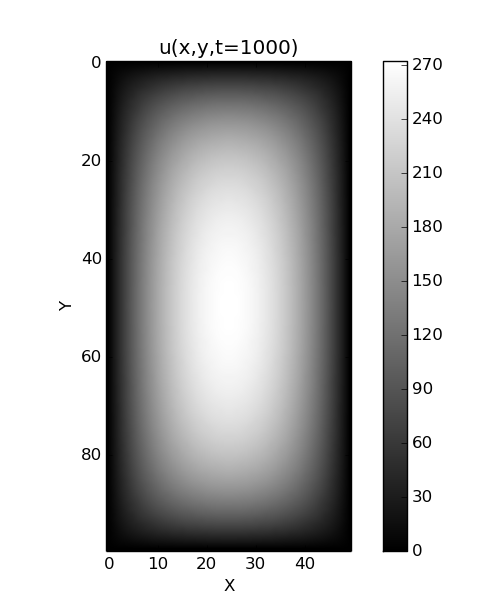
\includegraphics[width=0.5\textwidth]{purepython_res.png}
\caption{\label{FIG:purepython_res}Temperature distribution [Pure Python-solver]}
\end{figure}

\section*{5.2 Numpy and C implementations}
\subsection*{Numpy}
In stead of computing the terms one-by-one as done in 5.1, we can compute the whole 2D-matrix (called an array) at once and thus get rid of the loop over x and y-coordinate. This is done by vectorization of the code. One important thing to keep in mind, is that we want to exclude the boundary points. This means we have to pick out only the inner points and is done with the slice [1:-1,1:-1]. Note that we can use "comma" between the indices. Here we choose all x- and y-values starting from the second element and up to, but not included, the last one (index "-1"). When our update formula (\ref{EQ:upd_formula}), says $\pm$ 1 on an index, we have to move the entire slice the same. This can be seen in the code below:
\newline

\begin{minted}[bgcolor=LightGray, linenos, fontsize=\footnotesize]{python}
while t < t_end:
    u[1:-1,1:-1] = u[1:-1,1:-1] \
                 + dt*nu*(u[:-2,1:-1] + u[1:-1,:-2] - 4*u[1:-1,1:-1] \
                 +        u[1:-1,2:]  + u[2:,1:-1]) +nu*f[1:-1,1:-1]
    t += dt # Jump to next timestep
\end{minted}

Since the right hand side is computed and then assigned to the left hand side in one big step, we do not need a copy of the solution at the next time step, like we did before. Combined, these two changes saves computation time (drastically!) and halves the memory usage. Nice!

\subsection*{Results, NumPy}
The results is element wise exactly equal to the Python implementation, so no new figure is really needed (see fig.\ref{FIG:purepython_res}). However, the time spent computing is drastically lower, as we'll see later.

\subsection*{C, via Weave}
A third way to implement the time loop, is to use another language than Python, like C, and then do the heavy calculations here. Then we need some way to bridge these two languages, and my decision ended up on using Weave from the SciPy-package. We can then write C-code as a string, and call it with the \texttt{weave.inline()}-function. The time loop (and mesh grid loops) now look a lot like they did in the pure python-implementation, as can be seen below:
\newline

\begin{minted}[bgcolor=LightGray, linenos, fontsize=\footnotesize]{c}
int t,i,j;
for (t=0; t*dt<t_end+dt; t++){
    for (i=1; i<Nu[0]-1; i++) {
       for (j=1; j<Nu[1]-1; j++) {
           UN2(i,j) = U2(i,j) \
                    + dt*(U2(i-1,j) + U2(i,j-1) - 4*U2(i,j) \
                    + U2(i,j+1) + U2(i+1,j)) + nu*F2(i,j);
       }
    }
    for (i=1; i<Nu[0]-1; i++) {
       for (j=1; j<Nu[1]-1; j++) {
           U2(i,j) = UN2(i,j);
       }
    }
}
\end{minted}

The C-code above is stored as a string called \texttt{code} and is then executed with the following Python-code, where we have to tell what should be interpreted as constants, arrays etc, in a list of string-names. Weave then automatically makes some new variables we can use, like the dimensions n and m, is Nu[0] and Nu[1] (has nothing to do with $\nu$ / \texttt{nu}) and a 2D-array \texttt{u} is called \texttt{U2}. Indices is separated by a comma as in NumPy, but the brackets are curly. After computing \texttt{u\_new}, I copy these values to \texttt{u} through a double for-loop, to be used in the next iteration. This might seem slow, but as we'll see later, "for loops" in C are \textit{very} fast, so this is just fine!
\newline

\begin{minted}[bgcolor=LightGray, linenos, fontsize=\footnotesize]{python}
code = "int t,i,j; (.....)"
weave.inline(code, ['t_end','dt', 'u', 'un','f', 'nu'])
\end{minted}

\subsection*{Results, C via Weave}
As before, we get the exact same values computed (for all n-times-m-elements) and therefore I'd still like to refer the reader to figure \ref{FIG:purepython_res}. The advantage is of course even better performance in terms of speed, as we are going to examine in the next sections.we are going to examine in the next sections.

\section*{5.3 Testing the solvers}
\subsection*{Accuracy}
From the animation and plots, we can see that the solvers behave reasonably (in a physical sense). While keeping the edges cooled and constant, the temperature rises gradually with time until a steady state is reached. But do we know that we actually have a mathematically correct solver? To check this, we use the analytical solution when we let $t\rightarrow \infty$ and have a manufactured source term $f$:

\begin{align}
f(x,y) &= \nu\left(\left(\frac{2\pi}{(m-1)}\right)^2 + \left(\frac{2\pi}{(n-1)}\right)^2\right)\sin\left(\frac{2\pi x}{(n-1)}\right)\sin\left(\frac{2\pi y}{(m-1)}\right)
\end{align}

\begin{align}
u_{exact}(x,y) &= \sin\left(\frac{2\pi x}{n-1}\right)\sin\left(\frac{2\pi y}{m-1}\right)
\end{align}

This is implemented in the file \texttt{tests.py} and can be run both directly or with py.test. If run directly, it will test what happens with the error in the computation, when the mesh grid is increased.
\newline

Since all of the solvers give the exact same level of accuracy (or discrepancy between the analytic and numericaly computed solution), I'll list four runs where I have started with a 10-by-20 grid and then doubled the size three times. This can be seen in table \ref{TAB:test}. Due to the pure python-version being way too slow, it is not used to generate this data.

What we can see from the tabular data is that the error in the computation seems to decrease linearly with increasing mesh points. Since we quadruple the total number of points each time, the error should reduce by a factor 4. This is also the case. 

\begin{table}[ht]
\centering
\begin{tabular}{|l|l|l|l|l|}
\hline
\textbf{n} & \textbf{m} & \textbf{Max error} & \textbf{Numpy {[}sec{]}} & \textbf{Weave {[}sec{]}} \\ \hline
10 & 20 & 3.5E-2 & 1.150 & 0.041 \\ \hline
20 & 40 & 7.8E-3 & 1.426 & 0.190 \\ \hline
40 & 80 & 1.8E-3 & 2.303 & 0.814 \\ \hline
80 & 160 & 4.5E-4 & 6.336 & 3.478 \\ \hline
\end{tabular}
\caption{Error and speed of solvers. dt = 0.1, t1 = 2000\label{TAB:test}}
\end{table}

\subsection*{Speed}
Let's take a look at the speed-up we get from using NumPy and C. I have started with a grid size of 5-by-10, and then doubled the points three times, but this time also including the pure python-version. The results are put into table \ref{TAB:test}.

\begin{table}[ht]
\centering
\begin{tabular}{|l|l|l|l|l|l|l|}
\hline
\textbf{n} & \textbf{m} & \textbf{Python only} & \textbf{Numpy} & \textbf{Speed-up} & \textbf{Weave} & \textbf{Speed-up} \\ \hline
5 & 10 & 0.307 sec & 0.513 sec & 0.6 X & 0.006 sec & 55 X \\ \hline
10 & 20 & 1.775 sec & 0.567 sec & 3,2 X & 0.002 sec & 93 X \\ \hline
20 & 40 & 8.400 sec & 0.656 sec & 13 X & 0.090 sec & 93 X \\ \hline
40 & 80 & 36.54 sec & 1.123 sec & 33 X & 0.402 & 91 X \\ \hline
\end{tabular}
\caption{Run time comparison with pure-python-version. dt = 0.1, t1 = 1000\label{FIG:test2}}
\end{table}

From this, we immediately see that the larger the grid size, the better speed-up we can gain from NumPy. Meanwhile C (through Weave) gives an almost constant 90 X-improvement, which is just impressive!

\section*{5.4 User interface}
When using the file \texttt{heat\_equation\_ui.py}, the user can specify almost any setting from the command line. If any (or few or none) arguments are given, the default values are used, which are the "basic settings" we declared above. 
In addition to the grid size, time step, and interval settings, the user can also use "-v" or "-verbose" to get more information throughout the computation. Also, for time measurements "-time A B" can be given and this will make the program run the timeit-module A tests with each, B iterations. The total number of runs will be A times B.
\newline

The perhaps most important setting, is the choice of solver. Since only one might be used at the time, the user is only allowed to specify either "-python", "-numpy" or "-weave". If no argument is given, weave is used for its consistent speed. To save the last solution use "-s" or "-save". To output the last solution (as an array of numbers) use "-o FILENAME". If you wish to use this as a starting point for a new calculations, specify "-i FILENAME". A test will make sure that the dimensions agree. The user can also run:\\
\texttt{>>> python heat\_equation\_ui.py -h}\\
to get a full documentation of possibilities.

\section*{5.6 More interfaces}
\subsection*{C via Instant}
In the file \texttt{heat\_equation\_instant.py} I have used Instant to interface C-code in Python. The tricky part here is that you have to list both the dimensions and the arrays string-name to the inline-function. I add the variables dt, $\nu$ and t1 directly into the C-code via the $\%f$-python syntax.

\begin{minted}[bgcolor=LightGray, linenos, fontsize=\footnotesize]{python}
c_code      = """
  void heateq(int ux, int uy, double* u, int unx, int uny, \
	      double* un, int fx, int fy, double* f){
  double dt = %f;
  double nu = %f;
  double t_end = %f;
  int t,i,j;
  for (t=0; t*dt<t_end+dt; t++){
    (...)
  }
}"""%(dt,nu,t_end) # Add these values into C-code "as text"

heateq_func = inline_with_numpy(c_code, arrays = [['ux',  'uy',  'u' ],
                                                  ['unx', 'uny', 'un'],
                                                  ['fx',  'fy',  'f']])
heateq_func(u,un,f) # Run through all time steps in C
\end{minted}

When run directly, we get the same solution for u as we did earlier. Since we already have tested this solution to be valid, the Instant-interface is also validated. 

\end{document}



















